
\documentclass{beamer}
\usecolortheme{dove}
\setbeamertemplate{navigation symbols}{}
\usepackage{amsmath,amssymb,amsfonts,amsthm, multicol, subfigure, color}
\usepackage{bm}
\usepackage{graphicx}
\usepackage{tabularx}
\usepackage{booktabs}
\usepackage{hyperref}
\usepackage{pdfpages}
\usepackage{xcolor}
\definecolor{seagreen}{RGB}{46, 139, 87}
\definecolor{ucla}{RGB}{39, 116, 174}
\definecolor{darkestblue}{RGB}{0, 59, 92}
\definecolor{gold}{RGB}{255, 209, 0}
\def\independenT#1#2{\mathrel{\rlap{$#1#2$}\mkern2mu{#1#2}}}
\newcommand\indep{\protect\mathpalette{\protect\independenT}{\perp}}
\def\log{\text{log}}
\newcommand\logit{\text{logit}}
\newcommand\iid{\stackrel{\text{iid}}{\sim}}
\newcommand\E{\text{E}}
\newcommand\V{\text{V}}
\renewcommand\P{\text{P}}
\newcommand{\Cov}{\text{Cov}}
\newcommand{\Cor}{\text{Cor}}
\newcommand\doop{\text{do}}
\usepackage{stackrel}
\usepackage{tikz}
\usetikzlibrary{arrows,shapes.arrows,positioning,shapes,patterns,calc}
\newcommand\slideref[1]{\vskip .1cm \tiny \textcolor{gray}{{#1}}}
\newcommand\red[1]{\color{red}#1}
\newcommand\blue[1]{\color{blue}#1}
\newcommand\gray[1]{\color{gray}#1}
\newcommand\seagreen[1]{\color{seagreen}#1}
\newcommand\purple[1]{\color{purple}#1}
\newcommand\orange[1]{\color{orange}#1}
\newcommand\black[1]{\color{black}#1}
\newcommand\white[1]{\color{white}#1}
\newcommand\teal[1]{\color{teal}#1}
\newcommand\magenta[1]{\color{magenta}#1}
\newcommand\Fuchsia[1]{\color{Fuchsia}#1}
\newcommand\BlueGreen[1]{\color{BlueGreen}#1}
\newcommand\bblue[1]{\textcolor{blue}{\textbf{#1}}}
\newcommand\bred[1]{\textcolor{red}{\textbf{#1}}}
\newcommand\bgray[1]{\textcolor{gray}{\textbf{#1}}}
\newcommand\bgreen[1]{\textcolor{seagreen}{\textbf{#1}}}
\newcommand\bref[2]{\href{#1}{\color{blue}{#2}}}
\colorlet{lightgray}{gray!40}
\pgfdeclarelayer{bg}    % declare background layer for tikz
\pgfsetlayers{bg,main} % order layers for tikz
\newcommand\mycite[1]{\begin{scriptsize}\textcolor{darkgray}{(#1)}\end{scriptsize}}
\newcommand{\tcframe}{\frame{
%\small{
\only<1|handout:0>{\tableofcontents}
\only<2|handout:1>{\tableofcontents[currentsection]}}
%}
}

\usepackage[round]{natbib}
\bibliographystyle{humannat-mod}
\setbeamertemplate{enumerate items}[default]
\usepackage{mathtools}

\newcommand{\goalsframe}{\begin{frame}{Learning goals for today}
At the end of class, you will be able to estimate average causal effects by modeling treatment assignment probabilities. \vskip .2in
Optional reading:
\begin{itemize}
\item Hernán and Robins 2020 Chapter 12.1--12.5, 13, 15.1
\end{itemize}
\end{frame}}

\title{Doubly-Robust Estimation}
\author{Ian Lundberg\\Soc 212b\\\bref{https://ilundberg.github.io/soc212b}{ilundberg.github.io/soc212b}}
\date{Winter 2025}

\begin{document}

\maketitle

\goalsframe

\begin{frame}
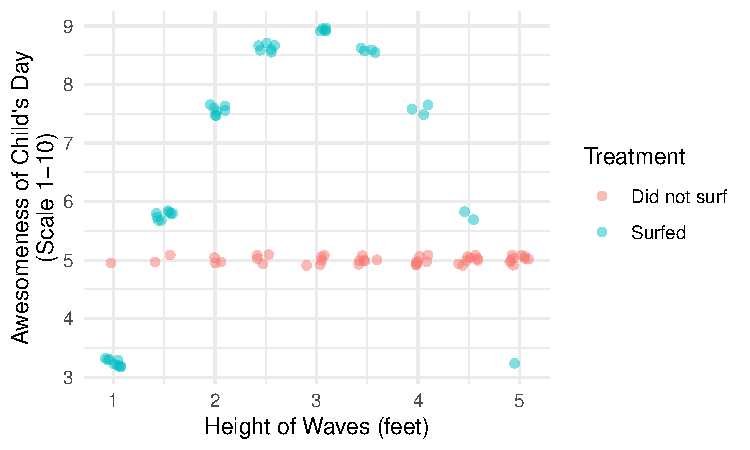
\includegraphics[width = \textwidth]{figures/dr_y.pdf}
\end{frame}

\begin{frame}
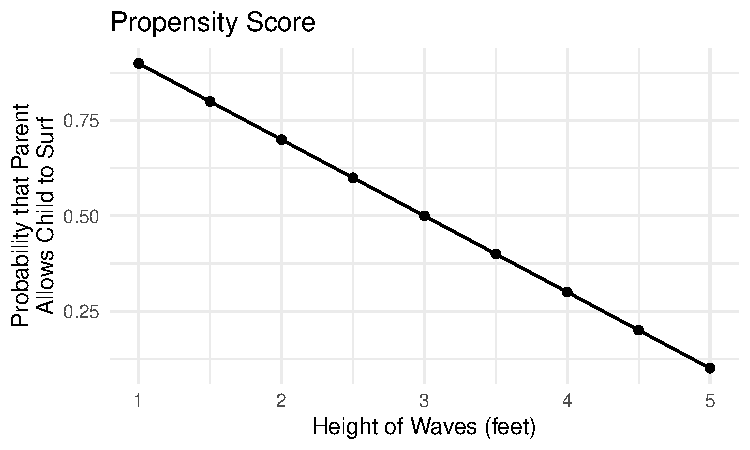
\includegraphics[width = \textwidth]{figures/dr_pscore.pdf}
\end{frame}

\begin{frame}

Child:\\How much more awesome would my day have been if I had surfed on the days when my parents didn't let me?
$$
\text{ATC} = \frac{1}{n_0}\sum_{i:A_i=0} \left(Y_i^1 - Y_i^0\right)
$$

\end{frame}

\begin{frame}

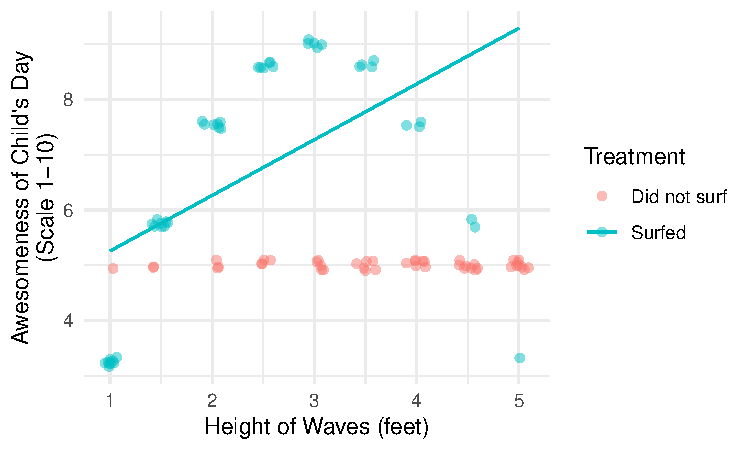
\includegraphics[width = \textwidth]{figures/dr_bestFitLine}

\end{frame}

\begin{frame}

\includegraphics[width = \textwidth]{figures/dr_predictedEffects}

\end{frame}

\begin{frame}

To discuss:
\begin{itemize}
\item In what sense is this line best-fit to the wrong goal?
\item How important is the error at each x-value?
\end{itemize}

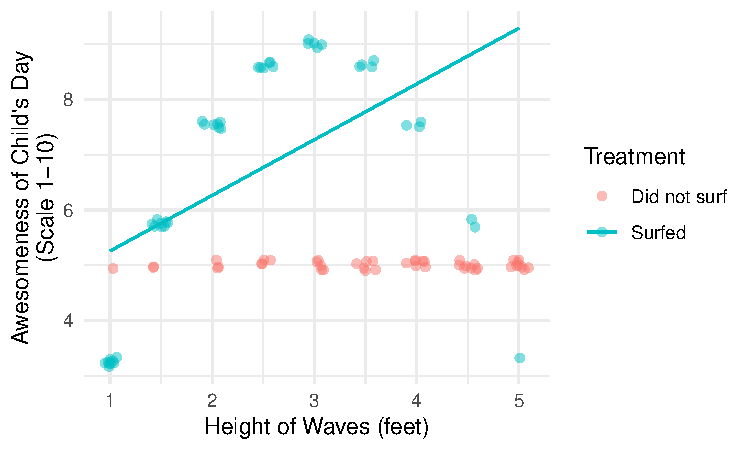
\includegraphics[width = \textwidth]{figures/dr_bestFitLine}

\end{frame}

\begin{frame}

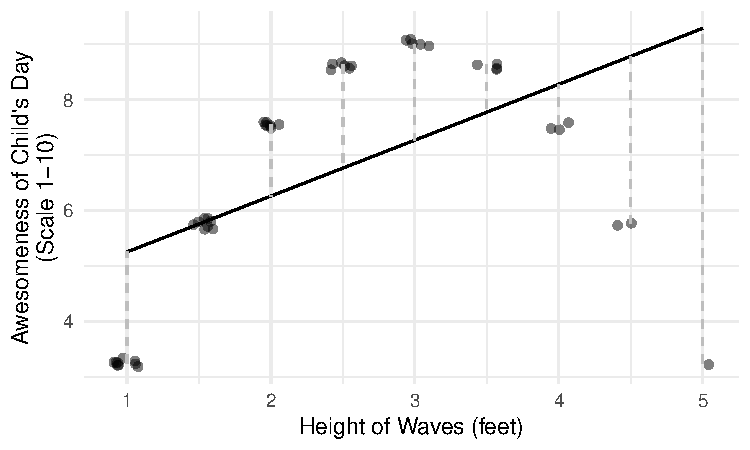
\includegraphics[width = \textwidth]{figures/dr_observedError}

\end{frame}

\begin{frame}

\onslide<2->{Weighted average error: 1.34.}\\
\onslide<3->{Corrected estimate: 2.94 - 1.34 = 1.60}

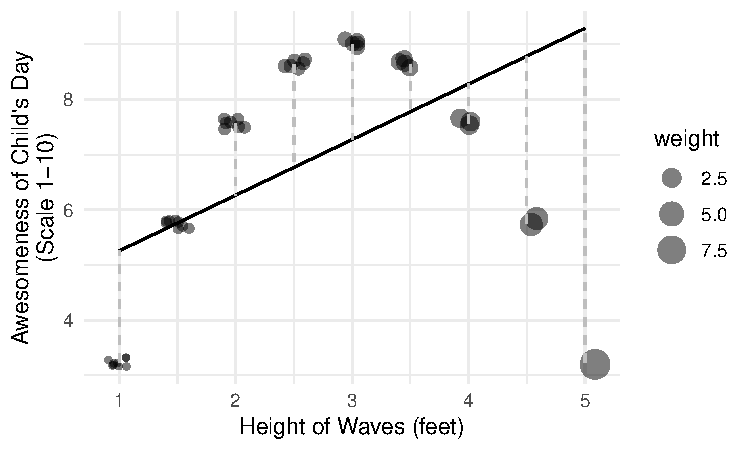
\includegraphics[width = \textwidth]{figures/dr_observedErrorWeighted}

\end{frame}

\begin{frame}{Doubly-robust estimation: Summary}

For the ATC:
\begin{itemize}
\item Predict $\hat{Y}^1$
\item Among treated cases,
\begin{itemize}
\item Weight by $\frac{\hat{P}(A = 1)}{\hat\P(A = 0)}$
\item Take weighted average error: $\hat{Y}^1 - Y$
\item This is a bias correction:\\model was fit at $x$-values of treated cases,\\target to predict is $x$-values of untreated cases
\end{itemize}
\item Among untreated cases, take average $\hat{Y}^1$
\item Then subtract the bias correction
\end{itemize}

\end{frame}

\goalsframe


\end{document}
